\textbf{COLUNI 2018 -- Questão 34}\par\medskip As figuras a seguir referem-se à tragédia do rompimento da barragem de Fundão, da empresa Samarco, no município de Mariana/MG e às suas consequências no município de Barra Longa/MG a jusante.

\par

\begin{center}
\begin{minipage}{0.48\linewidth}
\centering
Figura 1 - A lama atingindo Barra Longa\par
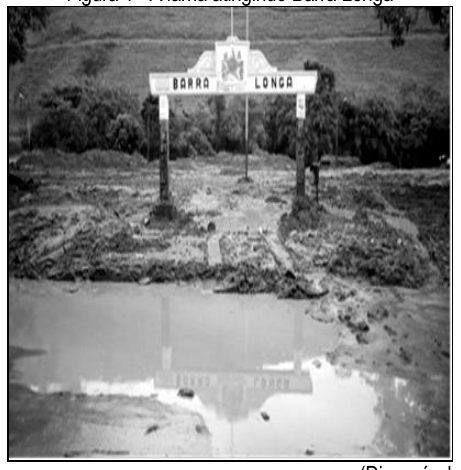
\includegraphics[width=\linewidth,trim=0 8pt 0 8pt,clip]{static/simulados/coluni/figuras/2018/questao-34/figura-1.png}
\end{minipage}\hfill
\begin{minipage}{0.48\linewidth}
\centering
Figura 2 - Deslocamento da lama capturado por imagem de satélite\par
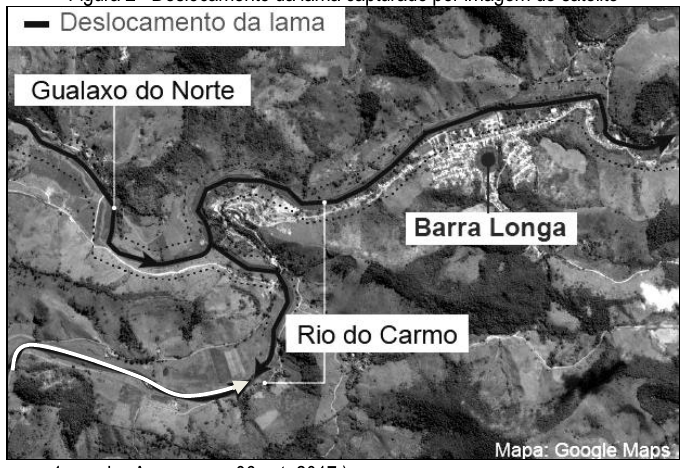
\includegraphics[width=\linewidth,trim=0 8pt 0 8pt,clip]{static/simulados/coluni/figuras/2018/questao-34/figura-2.png}
\end{minipage}\par
(Disponível em: www.g1.com.br. Acesso em: 06 set. 2017.)
\end{center}

Sobre as representações desta tragédia, nas figuras 1 e 2, é CORRETO afirmar:


\begin{enumerate}
\item A foto é o melhor instrumento para revelar os danos no município de Barra Longa.
\item A imagem de satélite está em escala cartográfica maior que a escala da foto.
\item A diferença escalar entre as figuras revela detalhes distintos da ação da lama.
\item A representação que mostra uma área menor é a imagem de satélite.
\end{enumerate}
